\documentclass[aspectratio=169]{beamer}
\usepackage{pgf}
\usepackage{multimedia}
\usepackage{colortbl,tabularx,mathrsfs,calligra,xcolor}
\usepackage{amsmath,amsfonts,amssymb,amsthm}
\usepackage{ragged2e}
\usepackage{setspace}
\usepackage{filecontents}
\usepackage{caption}
\usepackage{subcaption}
\usepackage{contour}
\usepackage{fancybox}
\usepackage{wrapfig}
\usepackage{multirow}
\usepackage{multicol}
\usepackage{pgfplots, tkz-euclide,calc}
    \usetikzlibrary{patterns,snakes,shapes.arrows}
\usepackage{listings}
\usepackage{enumitem}
\usepackage{pifont}
\usepackage[scaled]{berasans}
    \renewcommand*\familydefault{\sfdefault}  %% Only if the base font of the document is to be sans serif
\usepackage[T1]{fontenc}
\usepackage{hyperref}
\hypersetup{
    filecolor=magenta,      
    urlcolor=cyan,
    pdftitle={Overleaf Example},
    pdfpagemode=FullScreen,
    }
\renewcommand*\familydefault{\sfdefault} %% Only if the base font of the document is to be sans serif

\graphicspath{{C:/Users/teoso/OneDrive/Documents/Asisten Dosen & Lab/Asisten Laboratorium/Alpro 1/PPT/Graphicx/}}

\definecolor{HIMAmuda}{HTML}{01D1FD}
\definecolor{HIMAtua}{HTML}{02016A}
\definecolor{HIMAabu}{HTML}{CBCBCC}
\definecolor{PastelGreen}{HTML}{77DD77}
\definecolor{pgray}{rgb}{0.5,0.5,0.5}
\definecolor{pblue}{rgb}{0.13,0.13,1}
\definecolor{pgreen}{rgb}{0,0.5,0}
\definecolor{pred}{rgb}{0.9,0,0}
\definecolor{pgrey}{rgb}{0.46,0.45,0.48}
\definecolor{pcyan}{HTML}{D4EFFC}
\definecolor{lblue}{HTML}{00AEEF}
\definecolor{input}{HTML}{AAE1FA}
\definecolor{bg}{rgb}{0.95, 0.95, 0.92}
\definecolor{vscode}{HTML}{282A36}

\usetheme{Madrid}

\setbeamercolor{palette primary}{bg=HIMAtua,fg=white}
\setbeamercolor{palette secondary}{bg=HIMAmuda,fg=black}
\setbeamercolor{palette tertiary}{bg=HIMAabu,fg=black}
\setbeamercolor{palette quaternary}{bg=HIMAmuda,fg=white}
\setbeamercolor{structure}{fg=HIMAmuda} % itemize, enumerate, etc
\setbeamercolor{section in toc}{fg=HIMAtua} % TOC sections
\setbeamercolor{block title alerted}{fg=white,bg=magenta}
\setbeamercolor{block body alerted}{fg=black!90,bg=pink}

\usefonttheme{professionalfonts}
\setbeamertemplate{theorems}[numbered]
\setbeamertemplate{itemize items}[circle]

\usebackgroundtemplate{%
\tikz[overlay,remember picture] \node[opacity=0.1, at=(current page.center)]{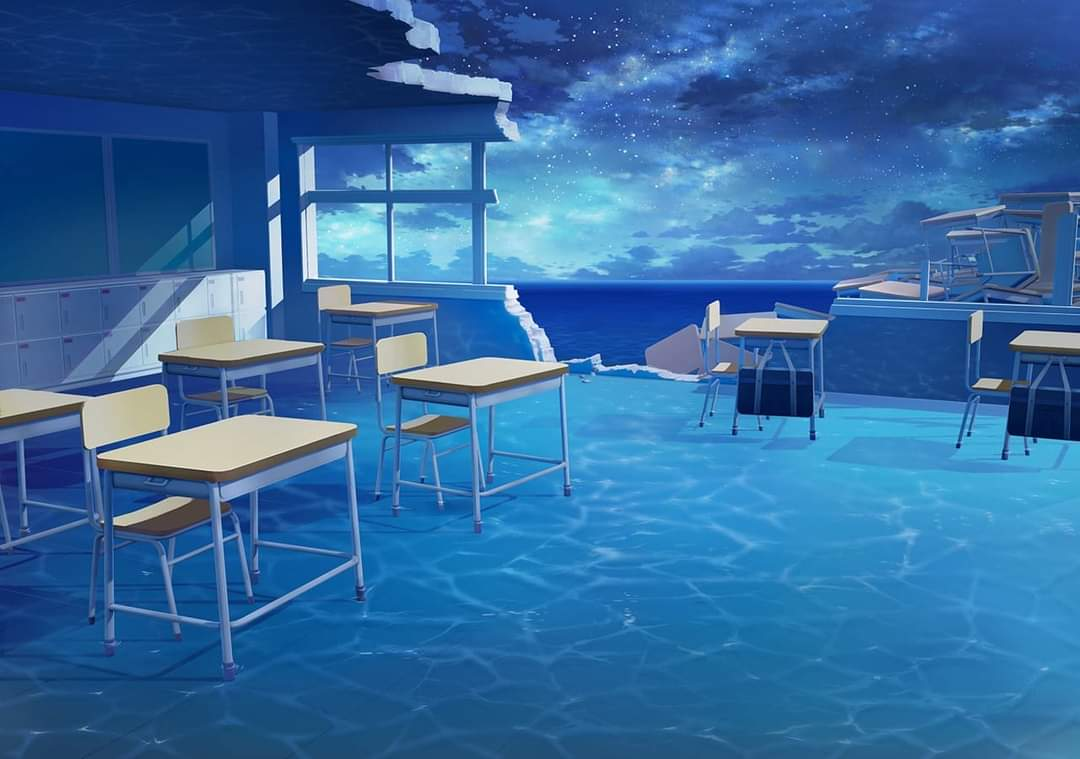
\includegraphics[width=\paperwidth]{plana class}};
}

\renewcommand\thesubfigure{\arabic{subfigure}}
\newtheorem*{funfact}{Fun Fact}
\newtheorem{latihan}{Latihan}
\newtheorem*{definisi}{Definisi}
\newtheorem{teorema}{Teorema}
\theoremstyle{definition}
\newtheorem*{contoh}{Contoh}
\newcommand{\R}{\mathbb{R}}

\AtBeginEnvironment{funfact}{%
  \setbeamercolor{block title}{fg=white,bg=PastelGreen} % Set title background to pastel green and text to white
  \setbeamercolor{block body}{parent=normal text,bg=PastelGreen!30!white} % Set body background to a lighter pastel green
}
\AtBeginEnvironment{definisi}{
    \setbeamercolor{block title}{fg=white,bg=HIMAtua}
    \setbeamercolor{block body}{parent=normal text,bg=HIMAtua!30!white}
}
\AtBeginEnvironment{teorema}{
    \setbeamercolor{block title}{bg=darkgray,fg=white}
    \setbeamercolor{block body}{parent=pallette tertiary,bg=HIMAabu!30!white}
}
\AtBeginEnvironment{latihan}{%
  \setbeamercolor{block title}{fg=white,bg=PastelGreen} % Set title background to pastel green and text to white
  \setbeamercolor{block body}{parent=normal text,bg=PastelGreen!30!white} % Set body background to a lighter pastel green
}

\renewcommand{\arraystretch}{1.3}

\usepackage{listings}

\lstdefinestyle{standard}{
    language            =Java,
    showspaces          =false,
    showtabs            =false,
    breaklines          =true,
    showstringspaces    =false,
    breakatwhitespace   =true,
    commentstyle        =\color{pgray},
    keywordstyle        =\color{pblue},
    stringstyle         =\color{pgreen},
    basicstyle          =\footnotesize\ttfamily,
    frame               =single,
    backgroundcolor     =\color{bg},
    escapeinside        ={(*}{*)},
    numbers             = left, % {none, left, right}
    numberstyle         = \scriptsize\color{black},
    numbersep           = -8pt,
    }

\lstdefinestyle{output}{
    language=Java,
    backgroundcolor=\color{vscode},
    basicstyle=\small\ttfamily\color{white},
    frame=none,
    escapeinside={(*}{*)},
    showspaces=false,
    showtabs=false,
    breaklines=true,
    showstringspaces=false,
    breakatwhitespace=true,
    }

\lstset{style=standard}

\author[Tew \& Haf]{Hafidz Mulia\\Teosofi Hidayah Agung}
\date{20 September 2024}
\title[Alpro 1 - Week 2]{Variabel}
\institute[Matematika ITS]{Departemen Matematika\\ Institut Teknologi Sepuluh Nopember}
\titlegraphic{{
\includegraphics[scale=0.02]{M.png}$\quad$
\includegraphics[scale=0.2]{Provicom.png}}}

\begin{document}
    {\usebackgroundtemplate{
        \tikz[overlay,remember picture] \node[opacity=0.2, at=(current page.center)]{
\includegraphics[width=\paperwidth]{bg_2}};}
    \begin{frame}
        \titlepage
    \end{frame}
    }

    \AtBeginSection{
    {\usebackgroundtemplate{
     \tikz[overlay,remember picture] \node[opacity=0.1, at=(current page.center)]{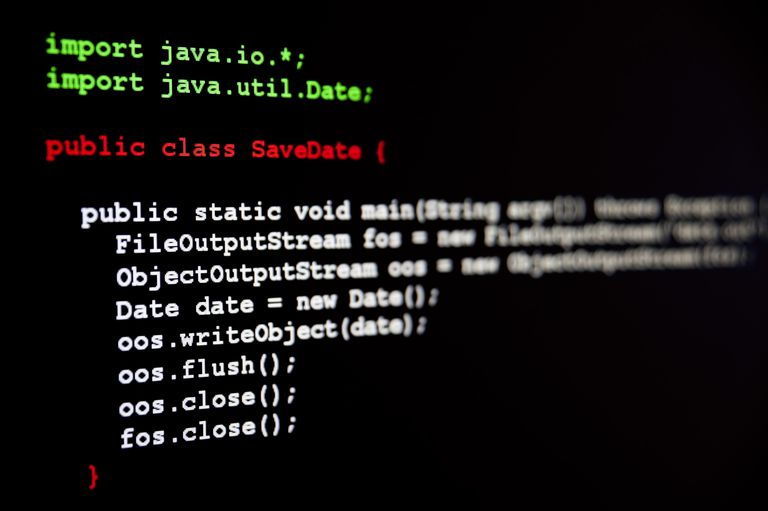
\includegraphics[width=\paperwidth]{Java code}};}
    \begin{frame}{Daftar isi}
        \tableofcontents[currentsection]
    \end{frame}}
    }

    \section{Variabel}
    {\usebackgroundtemplate{
        \tikz[overlay,remember picture] \node[opacity=0.1, at=(current page.center)]{
\includegraphics[width=\paperwidth]{motivated}};}
    \begin{frame}
        \frametitle{\insertsection}
        \begin{block}{Motivasi}
            Asumsikan kita ingin menggunakan komputer untuk mengetahui jawaban dari beberapa soal berikut:
            \begin{enumerate}[label=\arabic*.]
                \item Tentukan nilai dari $x$, jika $2x+4=5$.
                \item Jika $x=3$ dan $\displaystyle y=\frac{5}{3}$, maka tentukan nilai dari $xy$.
            \end{enumerate}
        \end{block}
        \onslide<2->{
        \begin{alertblock}{Penting}
            Selain dalam matematika, suatu \textcolor{red}{definisi} sangat penting untuk diperhatikan karena merupakan dasar dari suatu konsep yang akan dibangun nantinya. Dalam pemograman ini akan diajarkan tentang \textcolor{red}{deklarasi} dari suatu variabel.
        \end{alertblock}
        }
    \end{frame}
    }

    \begin{frame}
        \frametitle{\insertsection}
        \begin{definisi}
            Variabel atau peubah adalah suatu tempat penyimpanan yang digunakan untuk menyimpan nilai. Variabel terbagi menjadi dua jenis, yaitu variabel bebas dan variabel terikat. Variabel bebas adalah variabel yang nilainya dapat kita tentukan sendiri, sedangkan variabel terikat adalah variabel yang nilainya bergantung pada suatu fungsi.
        \end{definisi}
    \end{frame}

    \section{Tipe Data}
    \begin{frame}
        \frametitle{\insertsection}
        \begin{block}{Tipe Data}
            Suatu klasifikasi data yang memberikan informasi kepada kompiler atau interpreter bagaimana programmer bermaksud menggunakan data tersebut. Tipe data yang berbeda akan memungkinkan kita untuk melakukan operasi yang berbeda pada data tersebut.
        \end{block}
    \end{frame}

    {\setbeamercolor{block title}{bg=darkgray,fg=white}
    \setbeamercolor{block body}{parent=pallette tertiary,bg=HIMAabu!30!white}
    \begin{frame}
        \frametitle{\insertsection}
        \begin{columns}
            \begin{column}{0.45\textwidth}
                \begin{block}{\color{green}Primitif}
                    Tipe data dasar yang sudah disediakan oleh bahasa pemrograman. Tipe ini biasanya memiliki ukuran yang tetap dan langsung menyimpan nilai di memori.
                \end{block}
                \onslide<2->{
                \begin{exampleblock}{Contoh}
                    \begin{itemize}[label=$\blacksquare$]
                        \item \texttt{int}
                        \item \texttt{double}
                        \item \texttt{char}
                        \item \texttt{boolean}
                    \end{itemize}
                \end{exampleblock}
                }
            \end{column}
            \begin{column}{0.45\textwidth}
                \begin{block}{\color{cyan}Referensi}
                    tipe data yang mereferensikan lokasi memori di mana objek sebenarnya disimpan. Variabel tidak langsung menyimpan nilainya, melainkan menyimpan alamat ke nilai tersebut.
                \end{block}
                \onslide<2->{
                \begin{exampleblock}{Contoh}
                    \begin{itemize}[label=$\blacksquare$]
                        \item \texttt{String}
                        \item \texttt{Array}
                        \item \texttt{Class}
                        \item \texttt{Interface}
                    \end{itemize}
                \end{exampleblock}
                }
            \end{column}
        \end{columns}
    \end{frame}
    }

    \begin{frame}
        \frametitle{\insertsection}
        \begin{table}
            \centering
            \begin{tabular}{|c|c|c|}
                \hline
                \rowcolor{HIMAmuda}
                \textbf{Tipe Data} & \textbf{Ukuran} & \textbf{Default}\\
                \hline
                Boolean & 1 bit & false\\
                Byte & 1 byte & 0\\
                Short & 2 byte & 0\\
                Int & 4 byte & 0\\
                Long & 8 byte & 0L\\
                Float & 4 byte & 0.0\\
                Double & 8 byte & 0.0\\
                Char & 2 byte & \\
                \hline
            \end{tabular}
            \caption{Tipe Data Primitif}
        \end{table}
        {\footnotesize \textbf{Catatan}: 1 byte = 8 bit}
    \end{frame}

    \begin{frame}
        \frametitle{\insertsection}
        \begin{alertblock}{Perhatikan}
            Dalam mata kuliah ini, mungkin tidak terlalu mempedulikan ukuran dari tipe data. Namun, saat kita sudah terjun ke dalam dunia pemrograman yang lebih dalam, ukuran dari tipe data sangatlah penting untuk diperhatikan.
        \end{alertblock}
        \begin{figure}[h!]
            \centering
            \movie[width=0.5\textwidth,showcontrols,loop,borderwidth=0.5pt,start=7s,duration=9s,open,externalviewer]{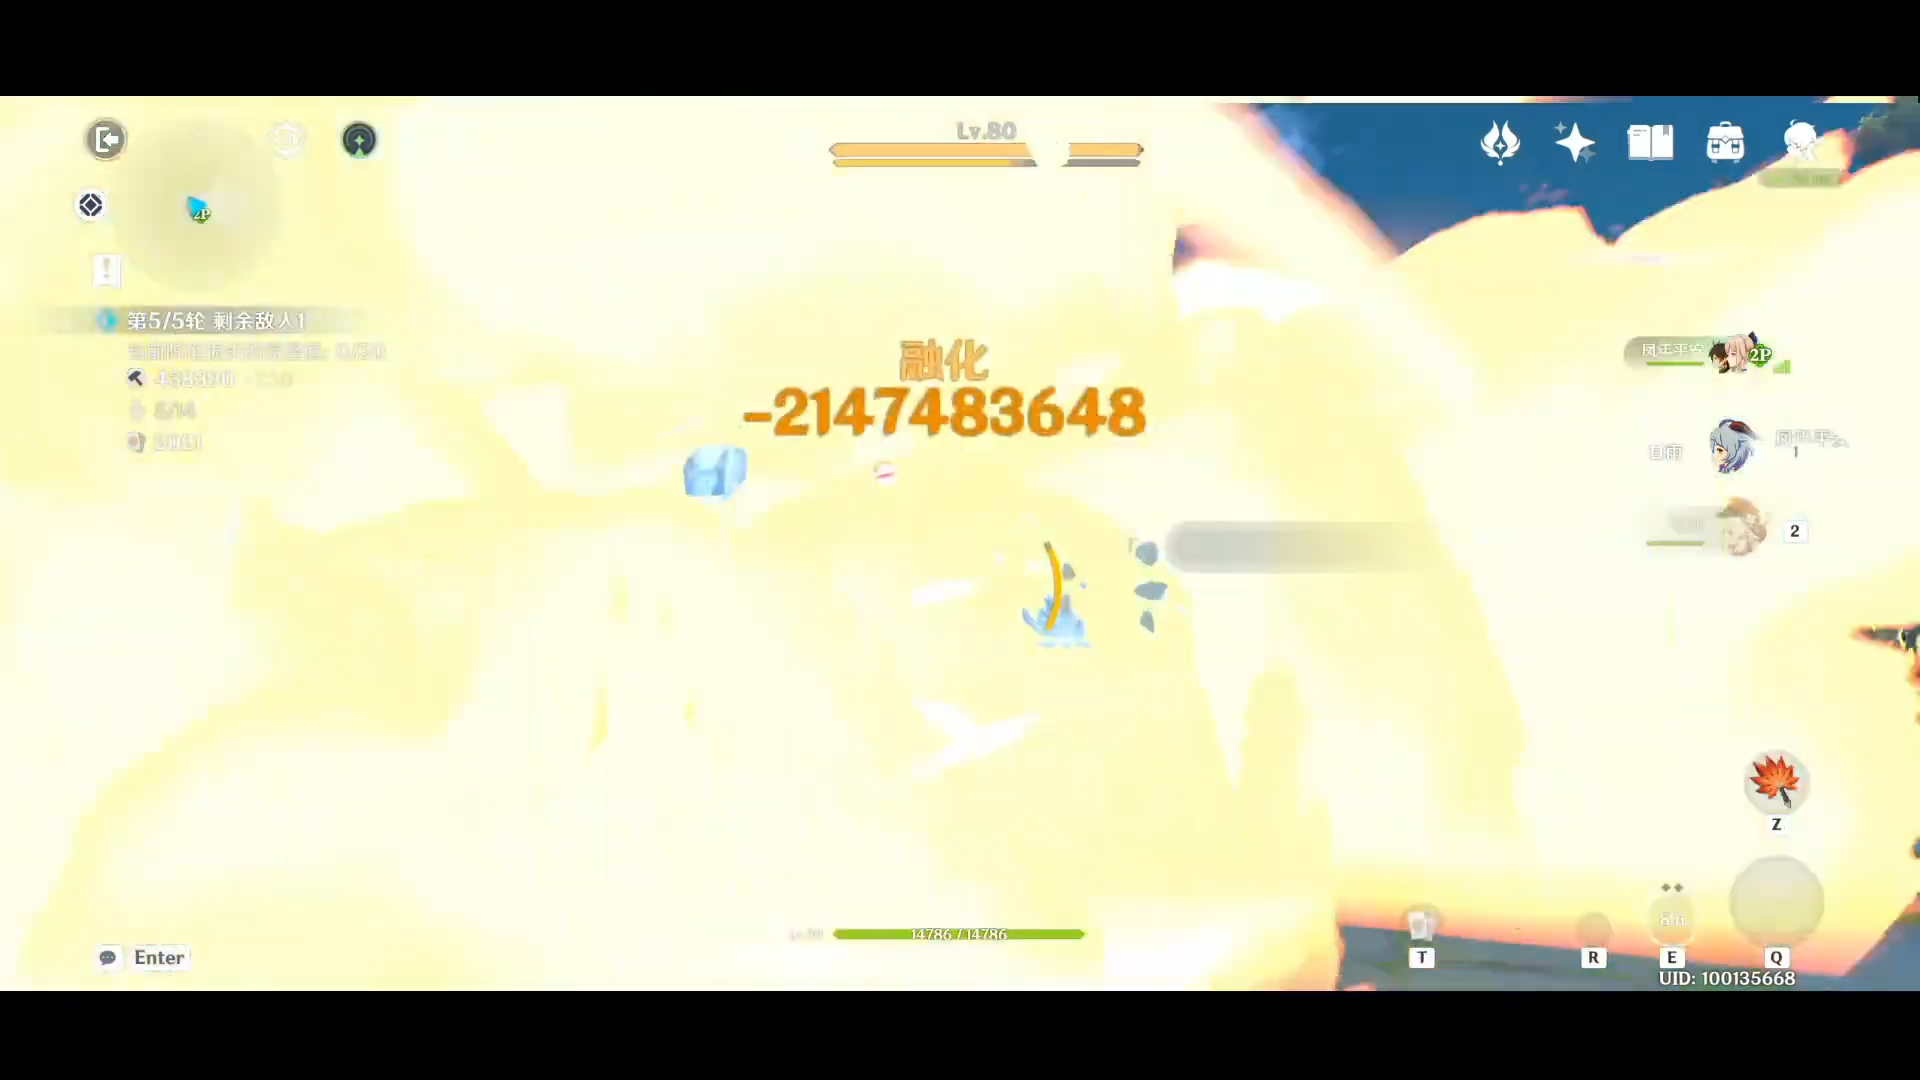
\includegraphics[width=0.5\textwidth,trim={0 3.3cm 0 3.5cm},clip]{genshin showcase}}{genshin.mp4}
            \caption*{YT Channel: \href{https://www.youtube.com/watch?v=wprBfd1aWG4}{\color{red} Tony To}}
        \end{figure}
    \end{frame}

    \section{Operator}
    \begin{frame}
        \frametitle{\insertsection}
        \begin{block}{Operator}
            Simbol yang digunakan untuk melakukan operasi tertentu pada variabel. Operator terbagi menjadi beberapa jenis, yaitu
            \begin{itemize}[label=$\circ$]
                \item \textbf{Operator Aritmatika}\\
                Operasi yang biasanya digunakan dalam matematika untuk menghasilkan suatu nilai.
                \item \textbf{Operator Boolean}\\
                Operasi yang biasanya digunakan dalam logika matematika untuk mengoperasikan antara dua nilai boolean.
                \item \textbf{Operator Relasional}\\
                Operasi yang digunakan untuk membandingkan dua nilai yang kemudian menghasilkan nilai boolean.
            \end{itemize}
        \end{block}
    \end{frame}

    \begin{frame}
        \frametitle{\insertsection}
        \begin{table}
            \centering
            \begin{tabular}{|c|c|c|}
                \hline
                \rowcolor{HIMAmuda}
                \textbf{Operator} & \textbf{Simbol} & \textbf{Contoh}\\
                \hline
                Penjumlahan & \texttt{+} & \texttt{a+b}\\
                Pengurangan & \texttt{-} & \texttt{a-b}\\
                Perkalian & \texttt{*} & \texttt{a*b}\\
                Pembagian & \texttt{/} & \texttt{a/b}\\
                Modulus & \texttt{\%} & \texttt{a\%b}\\
                \hline
            \end{tabular}
            \caption{Operator Aritmatika}
        \end{table}
    \end{frame}

    \begin{frame}
        \frametitle{\insertsection}
        \begin{table}
            \centering
            \begin{tabular}{|c|c|c|c|}
                \hline
                \rowcolor{HIMAmuda}
                & \multicolumn{2}{c|}{\textbf{Simbol}} & \\
                \cline{2-3}
                \rowcolor{HIMAmuda}
                \multirow{-2}{*}{\textbf{Operator}}& \textbf{Logika} & \textbf{Program} &\multirow{-2}{*}{\textbf{Contoh}} \\
                \hline
                \multirow{2}{*}{AND}& \multirow{2}{*}{$\land$} & \texttt{\&}& \texttt{a \& b}\\
                & & \texttt{\&\&}& \texttt{a \&\& b}\\
                \multirow{2}{*}{OR} & \multirow{2}{*}{$\lor$} & \texttt{|} & \texttt{a | b}\\
                & & \texttt{||} & \texttt{a || b}\\
                NOT & $\lnot$ & \texttt{!} & \texttt{!a}\\
                XOR & $\oplus$ & \texttt{\^} & \texttt{a \^\,b}\\
                \hline
            \end{tabular}
            \caption{Operator Boolean}
        \end{table}
    \end{frame}

    \begin{frame}
        \frametitle{\insertsection}
        \begin{table}
            \centering
            \begin{tabular}{|c|c|c|c|}
                \hline
                \rowcolor{HIMAmuda}
                & \multicolumn{2}{c|}{\textbf{Simbol}} & \\
                \cline{2-3}
                \rowcolor{HIMAmuda}
                \multirow{-2}{*}{\textbf{Operator}}& \textbf{Logika} & \textbf{Program} &\multirow{-2}{*}{\textbf{Contoh}} \\
                \hline
                Sama dengan & $=$ & \texttt{==} & \texttt{a == b}\\
                Tidak sama dengan & $\neq$ & \texttt{!=} & \texttt{a != b}\\
                Kurang dari & $<$ & \texttt{<} & \texttt{a < b}\\
                Lebih dari & $>$ & \texttt{>} & \texttt{a > b}\\
                Kurang dari sama dengan & $\leq$ & \texttt{<=} & \texttt{a <= b}\\
                Lebih dari sama dengan & $\geq$ & \texttt{>=} & \texttt{a >= b}\\
                \hline
            \end{tabular}
            \caption{Operator Relasional}
        \end{table}
    \end{frame}

    \section{Latihan}
    \begin{frame}[fragile]
        \begin{latihan}
            Menampilkan hasil beberapa operasi aritmatika dari dua variabel \texttt{a} dan \texttt{b}.
        \end{latihan}
        \begin{lstlisting}
    public class Latihan1{
        public static void main(String[] args){
            int a = 5;
            int b = 3;
            int c = a + b;
            int d = a - b;
            int e = a * b;
            System.out.println("Hasil dari " + a + " + " + b + " = " + c);
            System.out.println("Hasil dari " + a + " - " + b + " = " + d);
            System.out.println("Hasil dari " + a + " * " + b + " = " + e);
        }
    }
        \end{lstlisting}
    \end{frame}
    
    \begin{frame}[fragile]
        \begin{latihan}
            Buatlah sebuah program untuk melakukan sebuah konversi suhu dari celsius ke beberapa satuan yang lain (Kelvin, Reamur, Farenheit)!
            \begin{itemize}[label=$\bullet$]
                \item Celsius $(C)$ = $C$
                \item Kelvin $(K)$ = $C + 273$
                \item Reamur $(R)$ = $\displaystyle \frac{4}{5}\times C$
                \item Fahrenheit $(F)$ = $\displaystyle \frac{9}{5}\times C$
            \end{itemize}
        \end{latihan}
        \begin{lstlisting}[style=output,numbers=none]
Suhu dalam Celsius: 30
Suhu dalam Kelvin: 303
Suhu dalam Reamur: 24
Suhu dalam Fahrenheit: 86
        \end{lstlisting}
    \end{frame}
\end{document}